%%%%%%%%%%%%%%%%%%%%%%%%%%%%%%%%%%%%%%%%%%%%%%%%%%%%%%%%%%%%%%%%%%%%%%
% Template for a UBC-compliant dissertation
% At the minimum, you will need to change the information found
% after the "Document meta-data"
%
%!TEX TS-program = pdflatex
%!TEX encoding = UTF-8 Unicode

%% The ubcdiss class provides several options:
%%   gpscopy (aka fogscopy)
%%       set parameters to exactly how GPS specifies
%%         * single-sided
%%         * page-numbering starts from title page
%%         * the lists of figures and tables have each entry prefixed
%%           with 'Figure' or 'Table'
%%       This can be tested by `\ifgpscopy ... \else ... \fi'
%%   10pt, 11pt, 12pt
%%       set default font size
%%   oneside, twoside
%%       whether to format for single-sided or double-sided printing
%%   balanced
%%       when double-sided, ensure page content is centred
%%       rather than slightly offset (the default)
%%   singlespacing, onehalfspacing, doublespacing
%%       set default inter-line text spacing; the ubcdiss class
%%       provides \textspacing to revert to this configured spacing
%%   draft
%%       disable more intensive processing, such as including
%%       graphics, etc.
%%

% For submission to GPS
\documentclass[gpscopy,onehalfspacing,11pt]{ubcdiss}
\usepackage[margin=1in,
			left=1.1in]{geometry}
\makeatother


%!TEX root = MJThesis.tex
%%%%%%%%%%%%%%%%%%%%%%%%%%%%%%%%%%%%%%%%%%%%%%%%%%%%%____FONTS___%%%%%
%%
%% FONTS:
%% 
%% The defaults below configures Times Roman for the serif font,
%% Helvetica for the sans serif font, and Courier for the
%% typewriter-style font.  Configuring fonts can be time
%% consuming; we recommend skipping to END FONTS!
%% 
%% If you're feeling brave, have lots of time, and wish to use one
%% your platform's native fonts, see the commented out bits below for
%% XeTeX/XeLaTeX.  This is not for the faint at heart. 
%% (And shouldn't you be writing? :-)
%%

%% NFSS font specification (New Font Selection Scheme)
\usepackage{times,mathptmx,courier}
\usepackage[scaled=.92]{helvet}
\usepackage{sectsty}
\chapterfont{\usefont{T1}{qhv}{b}{n}\selectfont\huge}
%% Math or theory people may want to include the handy AMS macros
%\usepackage{amssymb}
%\usepackage{amsmath}
%\usepackage{amsfonts}
\usepackage{pifont, fixltx2e} % Adds \textsubscript{}, at least
\usepackage{titlesec} % titles! 
\usepackage{mhchem} % chemistry! \ce ;chem
\usepackage{float} % Floats! Now can use H as a placement option on floats.
\titleformat{\section}[hang]{
    \usefont{T1}{qhv}{b}{n}\selectfont} % "qhv" - TeX Gyre Heros, "b" - bold
    {} 
    {0em}
    {\hspace{-0.4pt}\Large \thesection\hspace{0.6em}}

%%%%%%%%%%%%%%%%%%%%%%%%%%%%%%%%%%%%%%%%%%%%%%%%%%%%%%____TOC___%%%%%
\usepackage{tocloft} % subfigure option only if using subfigure package
\renewcommand{\cfttoctitlefont} % ToC title
             {\usefont{T1}{qhv}{b}{n}\selectfont\huge}
\renewcommand{\cftchapfont} % chapter titles
             {\usefont{T1}{qhv}{b}{n}\selectfont}
\renewcommand{\cftsecfont} % section titles
             {\usefont{T1}{bch}{m}{n}\selectfont}
\renewcommand{\cftsubsecfont} % subsection titles
             {\usefont{T1}{bch}{m}{n}\selectfont} 
\renewcommand{\cftchappagefont} % chapter page numbers
             {\usefont{T1}{bch}{b}{n}\selectfont}
\renewcommand{\cftsecpagefont} % section page numbers
             {\cftsecfont} 
\renewcommand{\cftsubsecpagefont} % subsection page numbers
             {\cftsubsecfont}
%%%%%%%%%%%%%%%%%%%%%%%%%%%%%%%%%%%%%%%%%%%%%%%%____MICROTYPE___%%%%%
\usepackage[activate={true,nocompatibility},final,tracking=true,kerning=true,spacing=true,factor=1100,stretch=10,shrink=10]{microtype}
% activate={true,nocompatibility} - activate protrusion and expansion
% final - enable microtype; use "draft" to disable
% tracking=true, kerning=true, spacing=true - activate these techniques
% factor=1100 - add 10% to the protrusion amount (default is 1000)
% stretch=10, shrink=10 - reduce stretchability/shrinkability (default is 20/20)
\SetProtrusion{encoding={*},family={bch},series={*},size={6,7}}
              {1={ ,750},2={ ,500},3={ ,500},4={ ,500},5={ ,500},
               6={ ,500},7={ ,600},8={ ,500},9={ ,500},0={ ,500}}
\SetExtraKerning[unit=space]
    {encoding={*}, family={bch}, series={*}, size={footnotesize,small,normalsize}}
    {\textendash={400,400}, % en-dash, add more space around it
     "28={ ,150}, % left bracket, add space from right
     "29={150, }, % right bracket, add space from left
     \textquotedblleft={ ,150}, % left quotation mark, space from right
     \textquotedblright={150, }} % right quotation mark, space from left
\SetExtraKerning[unit=space]
   {encoding={*}, family={qhv}, series={b}, size={large,Large}}
   {1={-200,-200}, 
    \textendash={400,400}}
\SetTracking{encoding={*}, shape=sc}{20}   
\microtypecontext{spacing=nonfrench}        
%%%%%%%%%%%%%%%%%%%%%%%%%%%%%%%%%%%%%%%%%%%%%%%%%%%%%%%%%%%%%%%%%%%%%%
%%
%% Recommended packages
%%
\usepackage{checkend}	% better error messages on left-open environments
\usepackage{graphicx}	% for incorporating external images

%% booktabs: provides some special commands for typesetting tables as used
%% in excellent journals.  Ignore the examples in the Lamport book!
\usepackage{booktabs, multirow}
\usepackage{siunitx, xspace} %for SI units eg. \si{\grams\per\mega\hertz} and gives xspace

%% The acronym package provides support for defining acronyms, providing
%% their expansion when first used, and building glossaries.  See the
%% example in glossary.tex and the example usage throughout the example
%% document.
%% NOTE: to use \MakeTextLowercase in the \acsfont command below,
%%   we *must* use the `nohyperlinks' option -- it causes errors with
%%   hyperref otherwise.  See Section 5.2 in the ``LaTeX 2e for Class
%%   and Package Writers Guide'' (clsguide.pdf) for details.
\usepackage[printonlyused,nohyperlinks]{acronym}
%% The ubcdiss.cls loads the `textcase' package which provides commands
%% for upper-casing and lower-casing text.  The following causes
%% the acronym package to typeset acronyms in small-caps
%% as recommended by Bringhurst.
\renewcommand{\acsfont}[1]{{\scshape \MakeTextLowercase{#1}}}

%% color: add support for expressing colour models.  Grey can be used
%% to great effect to emphasize other parts of a graphic or text.
%% For an excellent set of examples, see Tufte's "Visual Display of
%% Quantitative Information" or "Envisioning Information".
\usepackage{color}
\definecolor{greytext}{gray}{0.5}
%%%%%%%%%%%%%%%%%%%%%%%%%%%%%%%%%%%%%%%%%%%%%%%%%%____COMMENT___%%%%%
%% comment: provides a new {comment} environment: all text inside the
%% environment is ignored.
%%   \begin{comment} ignored text ... \end{comment}
\usepackage{comment}

\titleformat*{\section}{\singlespacing\raggedright\bfseries\Large}
\titleformat*{\subsection}{\singlespacing\raggedright\bfseries\large}
\titleformat*{\subsubsection}{\singlespacing\raggedright\bfseries}
\titleformat*{\paragraph}{\singlespacing\raggedright\itshape}
%%%%%%%%%%%%%%%%%%%%%%%%%%%%%%%%%%%%%%%%%%%%%%%%%%____CAPTION___%%%%%
%% The caption package provides support for varying how table and
%% figure captions are typeset.
\usepackage[format=hang,indention=-1cm,labelfont={bf},margin=1em]{caption}

%% url: for typesetting URLs and smart(er) hyphenation.
%% \url{http://...} 
\usepackage{url}
\urlstyle{sf}	% typeset urls in sans-serif

%!TEX root = MJThesis.tex
%%%%%%%%%%%%%%%%%%%%%%%%%%%%%%%%%%%%%%%%%%%%%%%%%%%%%%%%%%%%%%%%%%%%%%
%% HYPERREF:
%% The hyperref package provides for embedding hyperlinks into your
%% document.  By default the table of contents, references, citations,
%% and footnotes are hyperlinked.
%%
%% Hyperref provides a very handy command for doing cross-references:
%% \autoref{}.  This is similar to \ref{} and \pageref{} except that
%% it automagically puts in the *type* of reference.  For example,
%% referencing a figure's label will put the text `Figure 3.4'.
%% And the text will be hyperlinked to the appropriate place in the
%% document.
%%
%% Generally hyperref should appear after most other packages

%% The following puts hyperlinks in very faint grey boxes.
%% The `pagebackref' causes the references in the bibliography to have
%% back-references to the citing page; `backref' puts the citing section
%% number.  See further below for other examples of using hyperref.
%% 2009/12/09: now use `linktocpage' (Jacek Kisynski): GPS now prefers
%%   that the ToC, LoF, LoT place the hyperlink on the page number,
%%   rather than the entry text.
%% The following is a directive for TeXShop to indicate the main file

\usepackage[hyperref=true,
            url=false,
            isbn=false,
            backref=true,
            style=custom-numeric-comp,
            citereset=chapter,
            maxcitenames=3,
            maxbibnames=100,
            backend=bibtex, % while checking on one of my (newest) systems, this option was needed to generate bibliography
            block=none]{biblatex}

    \usepackage{varioref}

    \usepackage[
		    bookmarksopen=true,
		    linktocpage=true,
		    urlcolor=linkcolor, % Color of URLs
		    citecolor=linkcolor, % Color of citations
		    linkcolor=linkcolor, % Color of links to other pages/figures
		    % backref=page,
		    pdfpagelabels=true,
		    plainpages=false,
		    % colorlinks=true, % Turn off all coloring by changing this to false
		    bookmarks=true,
		    pdfview=FitB]{hyperref}

		    %% The following change how the the back-references text is typeset in a
		    %% bibliography when `backref' or `pagebackref' are used
		    % \renewcommand\backrefpagesname{\(\rightarrow\) pages}
		    % \renewcommand\backref{\textcolor{greytext} \backrefpagesname\ }
    %%%%%%%%%%%%%%%%%%%%%%%%%%%%%%
    % Customisation
    %%%%%%%%%%%%%%%%%%%%%%%%%%%%%%
    % back reference text preceding the page number ("see p.")
    \DefineBibliographyStrings{english}{%
        backrefpage  = {see p.}, % for single page number
        backrefpages = {see pp.} % for multiple page numbers
    }

    % the followings activate 'custom-english-ordinal-sscript.lbx'
    % in order to print ordinal 'edition' suffixes as superscripts,
    % and adjusts (reduces) spacing between suffix and following "ed."
    \DeclareLanguageMapping{english}{custom-english-ordinal-sscript}
    \DeclareFieldFormat{edition}%
                       {\ifinteger{#1}%
                        {\mkbibordedition{#1}\addthinspace{}ed.}%
                        {#1\isdot}}

    % removes period at the very end of bibliographic record
    \renewcommand{\finentrypunct}{}

    % removes period after DOI and suppresses capitalization
    % of the word following DOI ("See p. xx" -> "see p. xx")
    \renewcommand{\newunitpunct}{\addspace\midsentence}

    \DeclareFieldFormat{journaltitle}{\mkbibemph{#1},} % italic journal title with comma
    \DeclareFieldFormat[inbook,thesis]{title}{\mkbibemph{#1}\addperiod} % italic title with period
    \DeclareFieldFormat[article]{title}{#1} % title of journal article is printed as normal text
    \DeclareFieldFormat[article]{volume}{\textbf{#1}\addcolon\space} % makes volume of journal bold and adds colon
    \DeclareFieldFormat{pages}{#1} % removes pagination (p./pp.) before page numbers
    %%%%%%%%%
% the command \upcite defined below prints footnote citation above punctuation
\newlength{\spc} % declare a variable to save spacing value
\newcommand{\upcite}[2][]{% new command with two arguments: optional (#1) and mandatory (#2)
        \settowidth{\spc}{#1}% set value of \spc variable to the width of #1 argument
        \addtolength{\spc}{-1.8\spc}% subtract from \spc about two (1.8) of its values making its magnitude negative
        #1% print the optional argument
        \hspace*{\spc}% print an additional negative spacing stored in \spc after #1
        \supershortnotecite{#2}}% print (cite) the mandatory argument
%%%%%%%%%
    % back reference text preceding the page number ("see p.")
    \DefineBibliographyStrings{english}{%
        backrefpage  = {see p.}, % for single page number
        backrefpages = {see pp.} % for multiple page numbers
    }
	%%%%%%%%%
	\usepackage{cleveref}
		\newcommand{\creflastconjunction}{, and\nobreakspace} %Oxford Comma for cref
    %%%%%%%%%
    % the followings activate 'custom-english-ordinal-sscript.lbx'
    % in order to print ordinal 'edition' suffixes as superscripts,
    % and adjusts (reduces) spacing between suffix and following "ed."
    \DeclareLanguageMapping{english}{custom-english-ordinal-sscript}
    \DeclareFieldFormat{edition}%
                       {\ifinteger{#1}%
                       {\mkbibordedition{#1}\addthinspace{}ed.}%
                       {#1\isdot}}    


%\usepackage{longtable}	% provide tables spanning multiple pages
%\usepackage{chngpage}	% support changing the page widths on demand
%\usepackage{tabularx}	% an enhanced tabular environment

%% enumitem: support pausing and resuming enumerate environments.
%\usepackage{enumitem}

%% ragged2e: provides several new new commands \Centering, \RaggedLeft,
%% \RaggedRight and \justifying and new environments Center, FlushLeft,
%% FlushRight and justify, which set ragged text and are easily
%% configurable to allow hyphenation.
%\usepackage{ragged2e}

%% The ulem package provides a \sout{} for striking out text and
%% \xout for crossing out text.  The normalem and normalbf are
%% necessary as the package messes with the emphasis and bold fonts
%% otherwise.
%\usepackage[normalem,normalbf]{ulem}    % for \sout

%% The following commands causes chapter and section references to
%% uppercase the part name.
\renewcommand{\chapterautorefname}{Chapter}
\renewcommand{\sectionautorefname}{Section}
\renewcommand{\subsectionautorefname}{Section}
\renewcommand{\subsubsectionautorefname}{Section}

%% If you have long page numbers (e.g., roman numbers in the 
%% preliminary pages for page 28 = xxviii), you might need to
%% uncomment the following and tweak the \@pnumwidth length
%% (default: 1.55em).  See the tocloft documentation at
%% http://www.ctan.org/tex-archive/macros/latex/contrib/tocloft/
% \makeatletter
% \renewcommand{\@pnumwidth}{3em}
% \makeatother

%%%%%%%%%%%%%%%%%%%%%%%%%%%%%%%%%%%%%%%%%%%%%%%%%%%%%%%%%%%%%%%%%%%%%%
%%%%%%%%%%%%%%%%%%%%%%%%%%%%%%%%%%%%%%%%%%%%%%%%%%%%%%%%%%%%%%%%%%%%%%
%%
%% Some special settings that controls how text is typeset
%%
% \raggedbottom		% pages don't have to line up nicely on the last line
% \sloppy		% be a bit more relaxed in inter-word spacing
% \clubpenalty=10000	% try harder to avoid orphans
% \widowpenalty=10000	% try harder to avoid widows
% \tolerance=1000

%% And include some of our own useful macros
% This file provides examples of some useful macros for typesetting
% dissertations.  None of the macros defined here are necessary beyond
% for the template documentation, so feel free to change, remove, and add
% your own definitions.
%
% We recommend that you define macros to separate the semantics
% of the things you write from how they are presented.  For example,
% you'll see definitions below for a macro \file{}: by using
% \file{} consistently in the text, we can change how filenames
% are typeset simply by changing the definition of \file{} in
% this file.
% 
%% The following is a directive for TeXShop to indicate the main file
%%!TEX root = diss.tex

\newcommand{\NA}{\textsc{n/a}}	% for "not applicable"

% Some useful macros for typesetting terms.
\newcommand{\file}[1]{\texttt{#1}}
\newcommand{\class}[1]{\texttt{#1}}
\newcommand{\latexpackage}[1]{\href{http://www.ctan.org/macros/latex/contrib/#1}{\texttt{#1}}}
\newcommand{\latexmiscpackage}[1]{\href{http://www.ctan.org/macros/latex/contrib/misc/#1.sty}{\texttt{#1}}}
\newcommand{\env}[1]{\texttt{#1}}
\newcommand{\BibTeX}{Bib\TeX}

% Define a command \doi{} to typeset a digital object identifier (DOI).
% Note: if the following definition raise an error, then you likely
% have an ancient version of url.sty.  Either find a more recent version
% (3.1 or later work fine) and simply copy it into this directory,  or
% comment out the following two lines and uncomment the third.
\DeclareUrlCommand\DOI{}
\newcommand{\doi}[1]{\href{http://dx.doi.org/#1}{\DOI{doi:#1}}}
%\newcommand{\doi}[1]{\href{http://dx.doi.org/#1}{doi:#1}}

% Useful macro to reference an online document with a hyperlink
% as well with the URL explicitly listed in a footnote
% #1: the URL
% #2: the anchoring text
\newcommand{\webref}[2]{\href{#1}{#2}\footnote{\url{#1}}}

% epigraph is a nice environment for typesetting quotations
\makeatletter
\newenvironment{epigraph}{%
	\begin{flushright}
	\begin{minipage}{\columnwidth-0.75in}
	\begin{flushright}
	\@ifundefined{singlespacing}{}{\singlespacing}%
    }{
	\end{flushright}
	\end{minipage}
	\end{flushright}}
\makeatother

% \FIXME{} is a useful macro for noting things needing to be changed.
% The following definition will also output a warning to the console
\newcommand{\FIXME}[1]{\typeout{**FIXME** #1}\textbf{[FIXME: #1]}}

%--------%% My Macros %%
\newcommand{\ecoli}{\ac{ecoli}\xspace}
\newcommand{\caulobacter}{\ac{caulobacter}\xspace}
\newcommand{\manB}{$\Delta$manB\xspace}
\newcommand{\done}{\hfill \checkmark}
\newcommand{\drsmit}{Dr.\,Smit\xspace}
\newcommand{\millilitre}{\si{\milli\litre}\xspace}
\newcommand{\microlitre}{\si{\micro\litre}\xspace}
\newcommand{\millimolar}{\si{\milli\molar}\xspace}
\newcommand{\micromolar}{\si{\micro\molar}\xspace}
\newcommand{\etal}{\textit{et\,al.}\xspace}
\newcommand{\dndc}[1][]{#1$\Delta{}$N$\Delta{}$C\xspace}
\newcommand{\cel}{\si{\degreeCelsius}\xspace}
\newcommand{\milligram}{\si{\milli\gram}\xspace}
\newcommand{\microgram}{\si{\micro\gram}\xspace}
\newcommand{\ie}{\textit{i.\!e.}~}
\newcommand{\del}{$\Delta{}$}
\newcommand{\mgperml}{\si{\milli\gram\per\milli\litre}\xspace}
\newcommand{\nanometer}{\si{\nano\meter}\xspace}
\newcommand{\eg}{\textit{e.\!g.}~}
\newcommand{\dr}{Dr.\,}
\newcommand{\phihind}{$\phi{}$29:\textit{Hin}DIII}
\newcommand{\lambdahind}{$\lambda$:\textit{Hin}DIII}
\newcommand{\tabr}{\ce{Ta6Br12^2+}\xspace}
\newcommand{\od}{\textsc{od}$_{600}$\xspace}


% END


%%%%%%%%%%%%%%%%%%%%%%%%%%%%%%%%%%%%%%%%%%%%%%%%%%%%%%%%%%%%%%%%%%%%%%
%%%%%%%%%%%%%%%%%%%%%%%%%%%%%%%%%%%%%%%%%%%%%%%%%%%%%%%%%%%%%%%%%%%%%%
%%
%% Document meta-data: be sure to also change the \hypersetup information
%%

\title{The structure, composition, and application of the cell envelope from \textit{Caulobacter crescentus}}
%\subtitle{If you want a subtitle}

\author{Michael D Jones}
\previousdegree{B. Science, Specialization in Biotechnology, University of Alberta, 2006}
\previousdegree{M. Science, Pharmaceutical Sciences, University of Alberta, 2008}

% What is this dissertation for?
\degreetitle{Doctor of Philosophy}

\institution{The University Of British Columbia}
\campus{Vancouver}

\faculty{The Faculty of Science}
\department{Microbiology and Immunology}
\submissionmonth{April}
\submissionyear{2015}

%% hyperref package provides support for embedding meta-data in .PDF
%% files
\hypersetup{
  pdftitle={The structure, composition, and application of the cell envelope of \textit{Caulobacter crescentus}  (DRAFT: \today)},
  pdfauthor={Michael D Jones},
  pdfkeywords={Your keywords here}
}

%%%%%%%%%%%%%%%%%%%%%%%%%%%%%%%%%%%%%%%%%%%%%%%%%%%%%%%%%%%%%%%%%%%%%%
%%%%%%%%%%%%%%%%%%%%%%%%%%%%%%%%%%%%%%%%%%%%%%%%%%%%%%%%%%%%%%%%%%%%%%
%% 
%% The document content
%%

%% LaTeX's \includeonly commands causes any uses of \include{} to only
%% include files that are in the list.  This is helpful to produce
%% subsets of your thesis (e.g., for committee members who want to see
%% the dissertation chapter by chapter).  It also saves time by 
%% avoiding reprocessing the entire file.
%\includeonly{intro,conclusions}
%\includeonly{discussion}
\addbibresource{biblio.bib} %%% Bibtex file
\begin{document}

%%%%%%%%%%%%%%%%%%%%%%%%%%%%%%%%%%%%%%%%%%%%%%%%%%
%% From Thesis Components: Tradtional Thesis
%% <http://www.grad.ubc.ca/current-students/dissertation-thesis-preparation/order-components>

% Preliminary Pages (numbered in lower case Roman numerals)
%    1. Title page (mandatory)
\maketitle

%    2. Abstract (mandatory - maximum 350 words)
%% The following is a directive for TeXShop to indicate the main file
%%!TEX root = diss.tex

\chapter{Abstract}

Classically, outer membranes are half lipid, half protein, and the outmost
layers of Gram-negative bacteria. For \textit{Caulobacter crescentus} the outer
membrane is the penultimate layer beneath a protein surface layer (S-layer). The
S-layer of the caulobacter cell envelope is an exciting platform for high
density peptide display and biotechnology development. We focused on elucidating
the structure of the outer membrane by crystallizing the S-layer protein, RsaA; solving the structure of the the lipopolysaccharide; and characterizing a newly discovered porin, OmpW. 

S-layer proteins are highly resistant to crystallization, because wo-dimensional
S-layer formation out competes three-dimensional crystal formation. To achieve a
crystallisable form of RsaA, a C-terminal truncation version was constructed and
expressed in the native host, \textit{C. crescentus}. The secreted protein was
prone to aggregation, so low agitation and slow concentration protocols had to
be developed. The RsaA truncate produced large crystals that diffracted to <2.5
\AA. Solving the phases proved to be a serious hurdle and the final protein structure remains unsolved.

The lipopolysaccharide of \textit{C. crescentus} is the anchor that supports the
S-layer. The structure of the lipid A portion was solved previously but
structures for the core oligosaccharide and the O-polysaccharide had not been deduced. In collaboration with Dr.\,Evgeny
Vinogradov, these remaining structures were solved.
The core oligosaccharide has a branched heptasaccharide structure. The O-polysaccharide is a heptasaccharide containing the dideoxy sugar N-acetylperosamine. Additionally, a rhamnan polysaccharide was discovered and its structure was determined. 

Porins, non-specific passive protein channels, are significant components of classical Gram-negative outer membranes. Despite this, no porin had ever been identified in \textit{C. crescentus}. We report the identification and characterization of the porin OmpW in \textit{C. crescentus}.  OmpW has low conductance of 125 pSv in 1 \si{\molar} \ce{KCl}. That is interesting because homologous porins in other bacteria have no detectable pore-forming activity.

The cell envelopes of bacteria are remarkable structures; the work here illuminates the unique structures present in the caulobacter envelope.

	\cleardoublepage

%    3. Preface
%% The following is a directive for TeXShop to indicate the main file
%%!TEX root = diss.tex

\chapter{Preface}

At UBC, a preface may be required.  Be sure to check the
GPSguidelines as they may have specific content to be included.

	\cleardoublepage

%    4. Table of contents (mandatory - list all items in the preliminary pages
%    starting with the abstract, followed by chapter headings and
%    subheadings, bibliographies and appendices)
\tableofcontents
	\cleardoublepage	% required by tocloft package

%    5. List of tables (mandatory if thesis has tables)
\listoftables
	\cleardoublepage	% required by tocloft package

%    6. List of figures (mandatory if thesis has figures)
\listoffigures
	\cleardoublepage	% required by tocloft package

%    7. List of illustrations (mandatory if thesis has illustrations)
%    8. Lists of symbols, abbreviations or other (optional)

%    9. Glossary (optional)
%% The following is a directive for TeXShop to indicate the main file
%%!TEX root = diss.tex

\DeclareAcronym{LPS}{
short = lps,long = lipopolysaccharide, 
short-format = \scshape}
\DeclareAcronym{PS}{
short = ps,long = polysaccharide, 
short-format = \scshape}
\DeclareAcronym{OPS}{
short = ops,long = O-specific polysaccharide, 
short-format = \scshape}
\DeclareAcronym{OS}{
short = os,long = oligosaccharide, 
short-format = \scshape}
\DeclareAcronym{UV}{
short = uv,long = ultraviolet Light, 
short-format = \scshape}
\DeclareAcronym{MALDI-TOF}{
short = maldi-tof,long = matrix assisted laser desorption/ionization-time of flight mass spectroscopy, 
short-format = \scshape}
\DeclareAcronym{S-layer}{
short = S-layer,long = protein surface layer, 
short-plural = {s}}
\DeclareAcronym{GC-MS}{
short = gc-ms,long = gas chromatography-mass spectroscopy, 
short-format = \scshape}
\DeclareAcronym{NMR}{
short = nmr,long = nuclear magnetic resonance spectroscopy, 
short-format = \scshape}
\DeclareAcronym{SDS-PAGE}{
short = sds-page,long = sodium dodecyl sulfate-polyacrylamide gel electrophoresis, 
short-format = \scshape}
\DeclareAcronym{PBS}{
short = pbs,long = phosphate-buffered saline, 
short-format = \scshape}
\DeclareAcronym{EDTA}{
short = edta,long = ethylenediaminetetraacetic acid, 
short-format = \scshape}
\DeclareAcronym{COSY}{
short = cosy,long = correlation spectroscopy, 
short-format = \scshape}
\DeclareAcronym{OD600}{
    short = \textsc{od}$_{600}$ ,
    long = optical density at 600 \si{\nano\metre} 
}
\DeclareAcronym{PCR}{
    short = pcr ,
    long = polymerase chain reaction, 
    short-format = \scshape 
}
\DeclareAcronym{gCOSY}{
short = g\textsc{cosy}, long = gradient correlation spectroscopy}
\DeclareAcronym{TOCSY}{ 
short = tcosy, long = total correlation spectroscopy,
short-format = \scshape}
\DeclareAcronym{PC}{
    short = pc,
    long = phosphatidylcholine, 
    short-format = \scshape}
\DeclareAcronym{ROESY}{
short = roesy,long = rotating frame nuclear Overhauser effect spectroscopy, 
short-format = \scshape}
\DeclareAcronym{HSQC}{
short = hsqc,long = heteronuclear single quantum coherence, 
short-format = \scshape}
\DeclareAcronym{gHSQC}{
short = g\textsc{hsqc}, long = gradient heteronuclear singe quantum coherence}
\DeclareAcronym{HMBC}{
short = hmbc,long = heteronuclear multiple bond coherence, 
short-format = \scshape}
\DeclareAcronym{gHMBC}{
short = g\textsc{hmbc}, long = gradient heteronuclear multiple bond coherence}
\DeclareAcronym{NOE}{
short = noe,long = nuclear Overhauser enhancement, 
short-format = \scshape}
\DeclareAcronym{NOESY}{
short = noesy, long = nuclear Overhauser enhancement spectroscopy, 
short-format = \scshape}
\DeclareAcronym{HMQC}{
short = hmqc,long = heteronuclear multiple-quantum correlation spectroscopy,
short-format = \scshape}
\DeclareAcronym{TLC}{
short = tlc,long = thin-layer chromatography, 
short-format = \scshape}
% \DeclareAcronym{ABC}{
% short = abc,long = ATP-binding cassette, 
% short-format = \s
% cshape}
\DeclareAcronym{EPS}{
short = eps,long = extracellular polysaccharide, 
short-format = \scshape}
\DeclareAcronym{PYE}{
    short = pye,
    long = peptone-yeast extract medium, 
    short-format = \scshape}
\DeclareAcronym{LDAO}{
    short = ldao ,
    long = lauryldimethylamine-oxide, 
    short-format = \scshape}
\DeclareAcronym{ESI}{
short = esi,long = electrospray ionization, 
short-format = \scshape}
\DeclareAcronym{TFA}{
short = tfa,long = trifluoroacetic acid, 
short-format = \scshape}
\DeclareAcronym{caulobacter}{
    short = C.\,crescentus,
    long = \textit{Caulobacter crescentus}, 
    short-format = \textit,
    class = bacteria
}
\DeclareAcronym{ecoli}{
    short = E.\,coli,
    long = \textit{Escherichia coli}, 
    short-format = \textit,
    class = bacteria
}
\DeclareAcronym{pseudomonas}{
    short = P.\,aeruginosa ,
    long = \textit{Pseudomonas aeruginosa} ,
    short-format = \textit,
    class = bacteria
}
 %%%%%%%--------------Sugars
\DeclareAcronym{man}{
    short = Man,
    long = mannose, 
    class = sugar
}
\DeclareAcronym{rha}{
    short = Rha ,
    long = rhamnose , 
    class = sugar
}
\DeclareAcronym{per}{
    short = PerN,
    long = perosamine , 
    class = sugar
}
\DeclareAcronym{glc}{
    short = Glc,
    long = glucose, 
    class = sugar
}
\DeclareAcronym{glca}{
    short = GlcA,
    long = glucuronic acid, 
    class = sugar
}
\DeclareAcronym{glcnac}{
    short = GlcNAc ,
    long = N-acetylglucosamine , 
    class = sugar
}
\DeclareAcronym{gala}{
    short = GalA,
    long = galacturonic acid, 
    class = sugar
}
\DeclareAcronym{hep}{
    short = Hep,
    long = heptose,
    class = sugar
}
\DeclareAcronym{glcome}{
    short = 3-O-MeGlc,
    long = 3-O-methylglucose, 
    class = sugar
}
\DeclareAcronym{MS}{
    short = ms,
    long = mass spectrometry, 
    short-format = \scshape
} 
\DeclareAcronym{kdo}{
    short = Kdo,
    long = ketodeoxyoctulosonic acid, 
    class = sugar
}
\DeclareAcronym{blast}{
    short = blast,
    long = Basic Local Alignment Search, 
    short-format = \scshape 
}
\DeclareAcronym{aa}{
    short = aa,
    long = amino acid, 
    short-format = \scshape 
}
\DeclareAcronym{cls}{
    short = cls,
    long = Canadian Light Source, 
    short-format = \scshape 
}
\DeclareAcronym{ssrl}{
    short = ssrl,
    long = Stanford Synchotron Radiation Light Source , 
    short-format = \scshape 
}
\DeclareAcronym{rtx}{
    short = rtx,
    long = repeat-in-toxin, 
    short-format = \scshape 
}
\DeclareAcronym{peg}{
    short = peg,
    long = polyethylene glycol, 
    short-format = \scshape 
}
\DeclareAcronym{mw}{
    short = mw,
    long = molecular weight, 
    short-format = \scshape 
}
\DeclareAcronym{pi}{
    short = pI,
    long = isoelectric point, 
}
\DeclareAcronym{t1ss}{
    short = t1ss ,
    long = type 1 secretion system, 
    short-format = \scshape 
}
\DeclareAcronym{abc}{
    short = abc ,
    long = \textsc{atp} binding cassette, 
    short-format = \scshape 
}
\DeclareAcronym{kd}{
    short = $K_D$ ,
    long = dissociation constant 
}
\DeclareAcronym{anthrax}{
    short = B.\,anthracis ,
    long = \textit{Bacillus anthracis}, 
    short-format = \itshape , 
    class = bacteria
}
\DeclareAcronym{aeromonas}{
    short = A.\,salmonicida ,
    long = \textit{Aeromonas Salmonicida}, 
    short-format = \itshape , 
    class = bacteria
}
\DeclareAcronym{cfetus}{
    short = C.\,fetus,
    long = \textit{Campylobacter fetus}, 
    short-format = \itshape , 
    class = bacteria
}
\DeclareAcronym{cfg}{
    short = cfg,
    long = Consortium of Functional Glycomics, 
    short-format = \scshape 
}
\DeclareAcronym{dls}{
    short = dls ,
    long = dynamic light scattering, 
    short-format = \scshape 
} 
\DeclareAcronym{salmonella}{
     short = S. typhimurium ,
    long = \textit{Salmonella typhimurium}, 
    short-format = \itshape , 
    class = bacteria
}
\DeclareAcronym{pma}{
    short = pma ,
    long = phorbol 12-myristate 13-acetate, 
    short-format = \scshape 
}
\DeclareAcronym{tnfa}{
    short = tnf-$\alpha$ ,
    long = tumor necrosis factor $\alpha$, 
    short-format = \scshape 
}
\DeclareAcronym{il}{
    short = il ,
    long = interleukin, 
    short-format = \scshape 
}
\DeclareAcronym{mcp1}{
    short = mcp-1 ,
    long = monocyte chemotactic protein 1, 
    short-format = \scshape 
}
\DeclareAcronym{ifnb}{
    short = ifn-$\beta$ ,
    long = interferon $\beta$, 
    short-format = \scshape
}
\DeclareAcronym{geo}{
    short = G. staerothermophilus ,
    long = \textit{Geobacillus stearothermophilus}, 
    short-format = \itshape , 
    class = bacteria
}	% always input, since other macros may rely on it
	\textspacing		% begin one-half or double spacing

%   10. Acknowledgements (optional)
%% The following is a directive for TeXShop to indicate the main file
%%!TEX root = diss.tex

\chapter{Acknowledgments}

First and most of all I'd like to thank my family. My parents, J.C. and Dorothea, your support has been completely indispensable. I am lucky to have such fantastic parents. My wife, Elizabeth, I started this PhD before I met you but I could not have finished it without you. 

I do believe I have had the best supervisory committee of anyone I know. Dr.\,Beatty, Dr.\,Murphy, and  Dr.\,Fernandez you have been the exactly perfect level of supportive, critical, and congratulatory. Thank you.

I have been incredibly fortunate to have been in the Smit lab. It has been said that choosing your supervisor is the most important choice you have to make in grad school---I chose well in John Smit. Dr.\,Smit, your patience with my crazy ideas let me grow as a scientist but your lack of patience with my crazy ideas kept me in line and prevented my PhD from lasting a decade. Dr.\,Nomellini, I have been fortunate to have you nearby to fix my mistakes, hear me complain about my mistakes, and showing me how to prevent future mistakes. The few other members of our lab that I have shared time with, Lyngrace, Jan, Christina, you have all been great allies in the lab.

Beyond the official credits that the are given, I want to acknowledge the incredible collaborators I have had since day one. 
Dr.\,Evgeny Vinogradov is the world's preeminent expert on bacterial polysaccharide analysis, there is quite literally no one that would have been a better collaborator for our lipopolysaccharide work. The Consortium for Functional Glycomics Core H at Emory University were incredibly easy to work with and even though our results with them were ultimately negative, the service they provide is an invaluable asset to the field. Dr.\,Martine Caroff has been a surprisingly helpful source of expertise and critique, especially critique.

The Murphy lab in our department of Microbiology and Immunology is the go to collaborators for protein X-ray crystallography, my experiences are evidence to why that is. All of them (Angele, Meghan, Slade, Jason, Catherine, Stephanie, Marek, Michael, Mariko) accepted me like a lab member from the start. Dr.\,Anson Chan was an exceptional partner for crystallography, his expertise kept us moving forward against a tough project. Especially I would like to thank Dr.\,Chan for staying up all night many times on our long data collection runs. Staying up late is not so bad, but staying up late for poor results deserves commendation. 

Dr.\,Roland Benz was my only collaborator to initiate a collaboration with us. The porin project started as a side-project but it has become a nice little story that I am happy to have been apart of. Dr.\,Benz, I hope to actually meet you one day.

Lastly, I would like to acknowledge my department as a whole. This department has been incredibly supportive and warm. With people like Darlene, Sue, and Dr.\,Gold guiding the ship, I never felt like we were going to crash. A special acknowledgment goes to Dr.\,Jan Burian, who was always around with encouragement and advice but especially for his organization of many departmental events and teams that brought together a cadre of scientists on the dodgeball court, on the softball diamond, and beyond the confines of campus.



%   11. Dedication (optional)

% Body of Thesis (not all sections may apply)
\mainmatter

	\acresetall	% reset all acronyms used so far

%    1. Introduction
%% The following is a directive for TeXShop to indicate the main file
%!TEX root = ../MJThesis.tex
\acresetall

\chapter{Introduction}
\label{ch:Introduction}

    \begin{epigraph}
            \emph{``But during the writing of this review, I learned how little I knew in this area, and this was a humbling and sobering experience. I am certain that I have made many mistakes due to my ignorance, and I hope that the review will be useful despite its many faults''}---~Hiroshi Nikaido (2003), my grand supervisor.
    \end{epigraph}

    \section{S-layer structure} % (fold)
    \label{sec:s_layer_structure}

        % \begin{comment}  % Notes on structure
        %         Notes on structure of S-layers:
        %             - Location (ref fig)
        %                 - anchor
        %             - Visual appearance 
        %                 - symmetry patterns (ref fig)
        %             - Protein vs glycoprotein
            %                 - protein specifics
        %             - Sequence gazing
        % \end{comment}

        \begin{figure}[p] % Cell envelopes diagrams
                \begin{center}
                    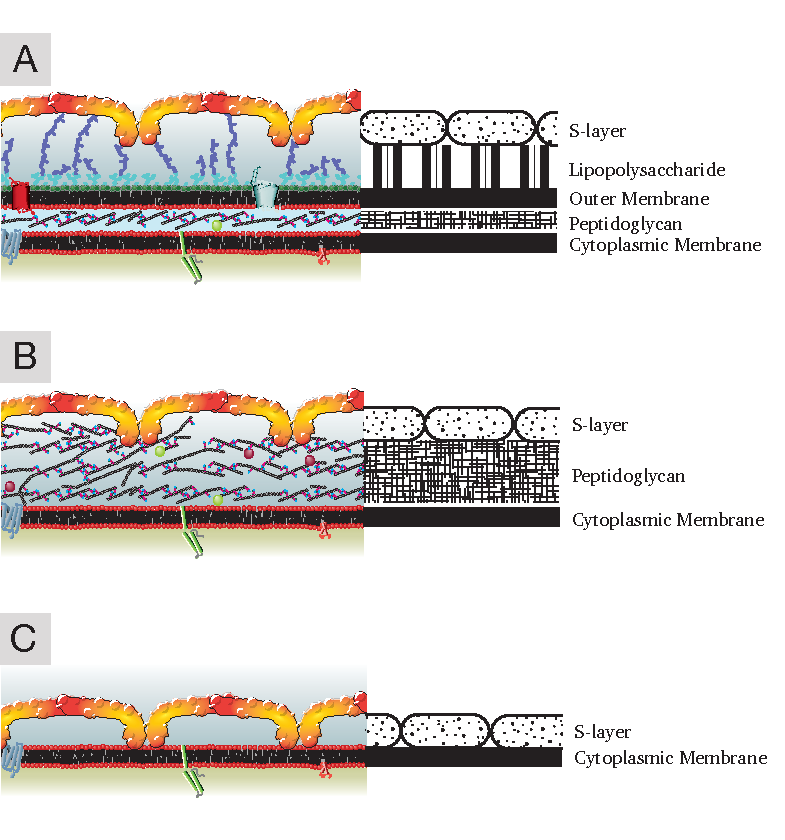
\includegraphics[]{intro/img/celwalls.pdf}
                \end{center}
                \caption[Cross-sectional diagrams of \ac{S-layer} containing cell envelopes]{Cross-sectional diagrams of the cell envelopes of (\textbf{A}) Gram negative bacteria, (\textbf{B}) Gram positive bacteria, and (\textbf{C}) archaebacteria. In all known cases the \ac{S-layer} sits on the extreme outer surface of the cell. (This diagram was inspired by Fig. 1 from \fullcite{sleytr1983crystalline})}
                \label{fig:cellwalls}
        \end{figure}

            Examples of bacteria with oblique \acs{S-layer} are \textit{Bacillus stearothermophilus} NRS2004$/$3a\upcite{messner1986characterization} and \textit{Lactobacillus brevis}\upcite[.]{masuda1980reassembly}
            Examples of bacteria with rectangular \acs{S-layer} are \textit{Corynebacterium diphtheriae}\upcite{kawata1972extracellular} and \textit{Aeromonas salmonicidae} A450\upcite[.]{ishiguro1981loss}
            An example of a bacterium with a triagonal \ac{S-layer} is \textit{Sulfolobus acidocaldarius}\upcite[.]{weiss1974subunit}
            Examples of bacteria with hexagonal \acs{S-layer} are \textit{Bacillus anthracis}\upcite{holt1969comparative} and \textit{Caulobacter crescentus}\upcite[.]{smit1981periodic}

        \begin{figure}[htb] % S-layer symmetries
                \begin{center}
                    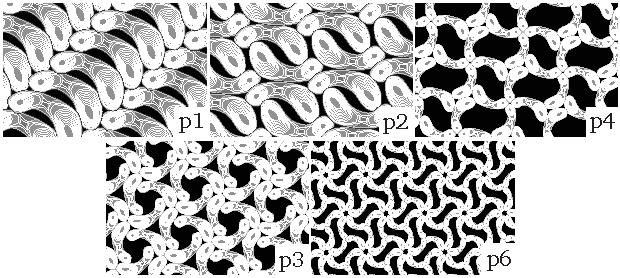
\includegraphics[]{intro/img/symmetries.pdf}
                \end{center}
                \caption[A simple overview of \ac{S-layer} symmetries]{A simple overview of \ac{S-layer} symmetries. p1 and p2 are oblique symmetries. 
                p4 is a rectangular symmetry.  
                p3  is a triagonal symmetry. 
                p6 is a hexagonal symmetry.}
                \label{fig:symmetries}
        \end{figure}


    % subsection s_layer_structure (end)

    \section{History of S-layers} % (fold)
    \label{sec:history_of_s_layers}
       
       % \begin{comment}  % Notes on history
       %      Notes on history of S-layers:
       %          - first seen
       %          - first cloned
       %          - first crystallised

       %      First (always) seen by EM

       %      First seen in Spirillum
       % \end{comment}

        \begin{figure}[p] % First S-layer
                \begin{center}
                    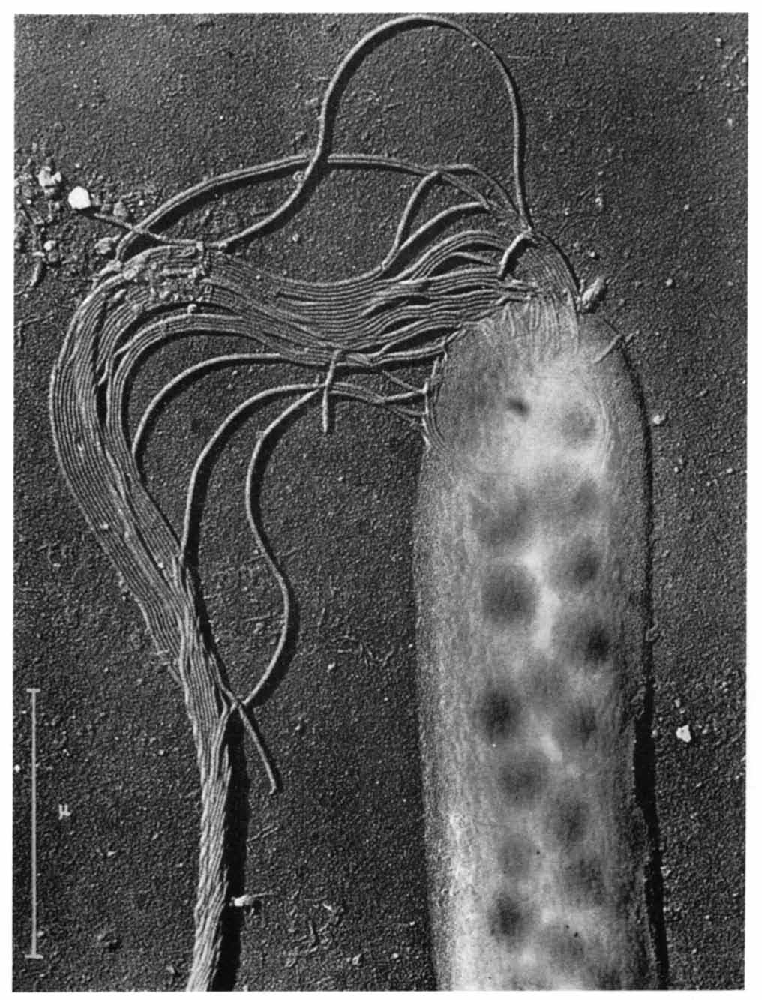
\includegraphics[]{intro/img/firstslayer.pdf}
                \end{center}
                \caption[The first published image of a \ac{S-layer}]{The first published image of a \ac{S-layer}. The hexagonal \ac{S-layer} on the surface of the bacterium --- probably \textit{Spirillum} sp. --- is visible along the edges of the cell body (centre right). The scale bar denotes one micrometre. (This image is Fig. 1 from \fullcite{firstslayer}, reused with full permission from the publisher, Elsevier.)}
                \label{fig:firstslayer}
        \end{figure}
    % section history_of_s_layers (end)
% section paracrystalline_protein_surface_layers (end)

\endinput

Any text after an \endinput is ignored.
You could put scraps here or things in progress.


%    2. Main body
% Generally recommended to put each chapter into a separate file
%\include{relatedwork}
%\include{model}
%\include{impl}
%\include{discussion}
%\include{conclusions}
%    3. Notes
%    4. Footnotes
%    5. Bibliography
% prints author names as small caps
\renewcommand{\mkbibnamefirst}[1]{\textsc{#1}}
\renewcommand{\mkbibnamelast}[1]{\textsc{#1}}
\renewcommand{\mkbibnameprefix}[1]{\textsc{#1}}
\renewcommand{\mkbibnameaffix}[1]{\textsc{#1}} 
\printbibliography[heading=bibintoc]

\appendix
%    6. Appendices (including copies of all required UBC Research
%       Ethics Board's Certificates of Approval)
%\include{reb-coa}	% pdfpages is useful here
\chapter*{Appendix}
% \section{The amino aid sequence of RsaA from \caulobacter}
\begin{figure}[htb]
  	\begin{center}
\label{app:rsaseq}
\texttt{\singlespacing\small\underline{MAYTTAQLVTAYTNANLGKAPDAATTLTLDAYATQTQTGGLSDAAALTNTLKLVNSTTAV}\hfill-60~~\\
\underline{AIQTYQFFTGVAPSAAGLDFLVDSTTNTNDLNDAYYSKFAQENRFINFSINLATGAGAGA}\hfill-120~\\
\underline{TAFAAAYTGVSYAQTVATAYDKIIGNAVATAAGVDVAAAVAFLSRQANIDYLTAFVRANT}\hfill-180~\\
\underline{PFTAAADIDLAVKAALIGTILNAATVSGIGGYATATAAMI}NDLSDGALSTDNAAGVNLFT\hfill-240~\\
AYPSSGVSGSTLSLTTGTDTLTGTANNDTFVAGEVAGAATLTVGDTLS\textbf{GGAGTDVLN}WVQ\hfill-300~\\
AAAVTALPTGVTISGIETMNVTSGAAITLNTSSGVTGLTALNTNTSGAAQTVTAGAGQNL\hfill-360~\\
TATTAAQAANNVAVDGGANVTVASTGVTSGTTTVGANSAASGTVSVSVANSSTTTTGAIA\hfill-420~\\
VTGGTAVTVAQTAGNAVNTTLTQADVTVTGNSSTTAVTVTQTAAATAGATVAGRVNGAVT\hfill-480~\\
ITDSAAASATTAGKIATVTLGSFGAATIDSSALTTVNLSGTGTSLGIGRGALTATPTANT\hfill-540~\\
LTLNVNGLTTTGAITDSEAAADDGFTTINIAGSTASSTIASLVAADATTLNISGDARVTI\hfill-600~\\
TSHTAAALTGITVTNSVGATLGAELATGLVFT\textbf{GGAGADSILL}GATTKAIVMGAGDDTVTV\hfill-660~\\
SSATLGAGGSVN\textbf{GGDGTDVLV}ANVNGSSFSADPAFGGFETLRVAGAAAQGSHNANGFTAL\hfill-720~\\
QLGATAGATTFTNVAVNVGLTVLAAPTGTTTVTLANATGTSDVFNLTLSSSAALAAGTVA\hfill-780~\\
LAGVETVNIAATDTNTTAHVDTLTLQATSAKSIVVTGNAGLNLTNTGNTAVTSFDASAVT\hfill-840~\\
GTGSAVTFVSANTTVGEVVTIR\textbf{GGAGADSLT}GSATANDTII\textbf{GGAGADTLV}YTGGTDTFT\textbf{G}\hfill-900~\\
\textbf{GTGADIFD}INAIGTSTAFVTITDAAVGDKLDLVGISTNGAIADGAFGAAVTLGAAATLAQ\hfill-960~\\
YLDAAAAGDGSGTSVAKWFQFGGDTYVVVDSSAGATFVSGADAVIKLTGLVTLTTSAFAT\hfill-1020\\
EVLTLA\hfill-1026\\
  }
   	\end{center}
   	\caption[RsaA, amino acid sequence]{
   The amino acid sequence of the \ac{S-layer} protein, RsaA from \caulobacter{} NA1000. GeneID:~\texttt{CCNA\_01059}. Ensembl Accession number: \texttt{ACL94524}. The encoding gene has the coordinates of 1 159 693 bp--1 162 773 bp on the forward strand of the \caulobacter chromosome. The underlined sequence corresponds to the amino acids 1--222, the section of the protein that was removed to generate a crystallizable C-terminal fragment. The bolded sequences are the \ac{rtx} motifs in RsaA. For the crystallization of RsaA, see \cref{ch:crystal} \cpageref{ch:crystal}.}
   	
\end{figure}   
% \section{The amino acid sequence of OmpW from \caulobacter}
\begin{figure}[htb]
  	\begin{center}
\label{app:ompwseq}
\texttt{\singlespacing\small  MKKLALSLVAFGALAAGAAQAQDFTPNAKGDLIVHARLTQVAPAKDAAILTAAGANSGLK\hfill-60~\\
AHVGNDIKPTLGFTYFLTDKVAVEAILGTTEHNIRAQGPGTDVLVHKTWVLPPVVTLQYH\hfill-120\\
PLPASQVSPYVGAGLNYMLFYSGKNKNGFTVKVDDGVGYALQAGVNIKMKNSWLVNADV\textbf{K}\hfill-180\\
KVYFSTDAKINGGALKAKVDLDPVVASIGLSRKF\hfill-214\\
  }
   	\end{center}
   	\caption[OmpW, amino acid sequence]{
   The amino acid sequence of the outer membrane channel, OmpW from \caulobacter NA1000. GeneID: \texttt{CCNA\_01475}. Ensembl Accession number: \texttt{ACL94940}. The encoding gene has the coordinates of 1 582 599 bp--1 583 243 bp on the forward strand of the \caulobacter chromosome. The bolded `K' is the location of the putative hydrophobic gate in \ecoli and \ac{pseudomonas}, where that residue encodes for a tryptophan; in \caulobacter that residue is a lysine. For our investigations into OmpW, see \cref{ch:porin} on \cpageref{ch:porin}}
\end{figure}   


\backmatter
%    7. Index
% See the makeindex package: the following page provides a quick overview
% <http://www.image.ufl.edu/help/latex/latex_indexes.shtml>


\end{document}
